\startchapter{Possibilities for treating experimental data} \label{ch:6}
\section{Description}
The experimental spectra obtained from IR, Raman or SFG techniques have an amplitude scaling factor when comparing to the candidate spectra generated mathematically. This means that between candidates' theoretical spectra and the experimental one, there is an unknown scaling factor. Within one particular spectroscopy technique, this scaling factor is the same for any polarization. Take IR as an example, the scaling factor for the spectrum of $x$ polarization is the same as the one for the spectrum of $z$ polarization. It is necessary to introduce this scaling factor to the LP models. The LP models constructed by Experiment 2 to 7 in Table \ref{tab:5.1} for $\theta$ ranged from $0^{\circ}$ to $80^{\circ}$) are doing well in retrieving the target composition for the mixed amino acids. Therefore, based on these experiments, we would like to know if the same LP models can be applied directly to the real experimental data for the same $\theta$ range.\\

Therefore, the same experiment setting in Table \ref{tab:5.1} are used for the following experiments. The goal is the same, to figure out which spectral information helps to retrieve the target composition for the mixture of six amino acids' candidates. The only difference is that, in each run of the experiment set, an arbitrary scaling factor is generated for IR, Raman and SFG, respectively. Therefore, the target spectra is not only composed by the target composition of all candidates, but also need to multiple by the randomly generated scaling factors of each spectroscopy technique. \\

To start with, we limit the scaling factors to be smaller than 1. \\

After a few runs of the experiment set, it is observed that the returned compositions always contains one extra variable in every experiment. For Experiment 2, 4, 6 and 7, the returned composition contains the right selected candidates. However, the percentage values of the candidates are different from the target composition. The ratio between the returned percentage and the target percentage are the same for the selected candidates. Furthermore, when this ratio adds up the extra variable, it equals $1$. Randomly select one experiment run, then take Experiment 2 as an example. Figure \ref{fig:6.2} displays the target composition generated, only the selected candidates are annotated with assigned percentage. Figure \ref{fig:6.2} displays the return composition of Experiment 2. The selected candidates in the return composition are in the right position, however, each percentage value is different from the one in the target composition. There are one extra value in Figure \ref{fig:6.2} whith value of $0.4$. \\

\begin{figure}[!ht] 
\centering
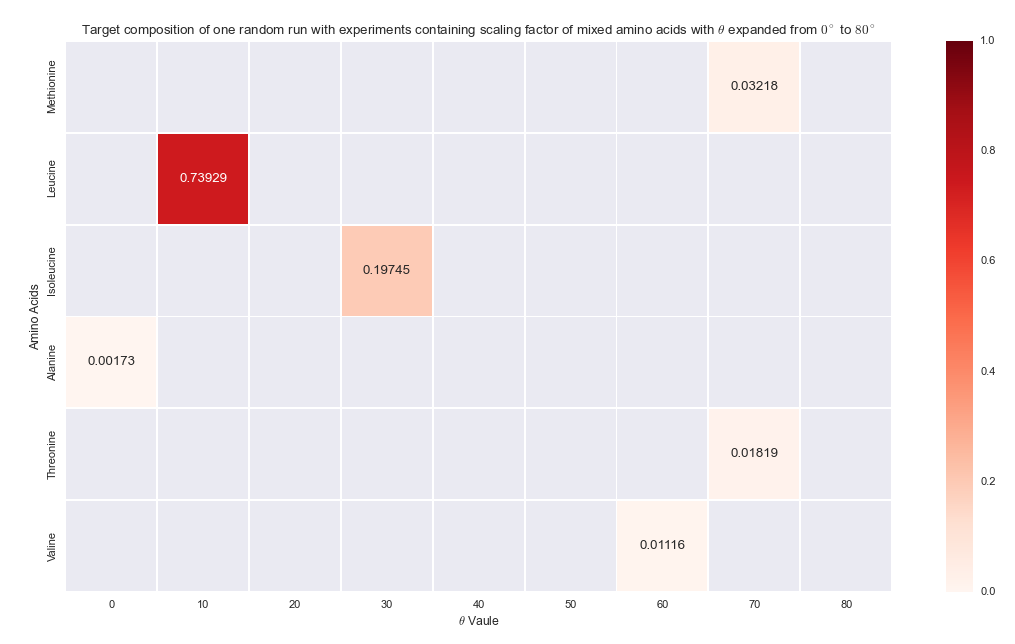
\includegraphics[scale=0.5]{Figures/chapter6_figure_one.png}
\caption{Target composition for one random run of experiment set with scaling foctor for mixed amino acids with $\theta$ expended from $0^{\circ}$ to $80^{\circ}$} \label{fig:6.1}
\end{figure}


\begin{figure}[!ht] 
\centering
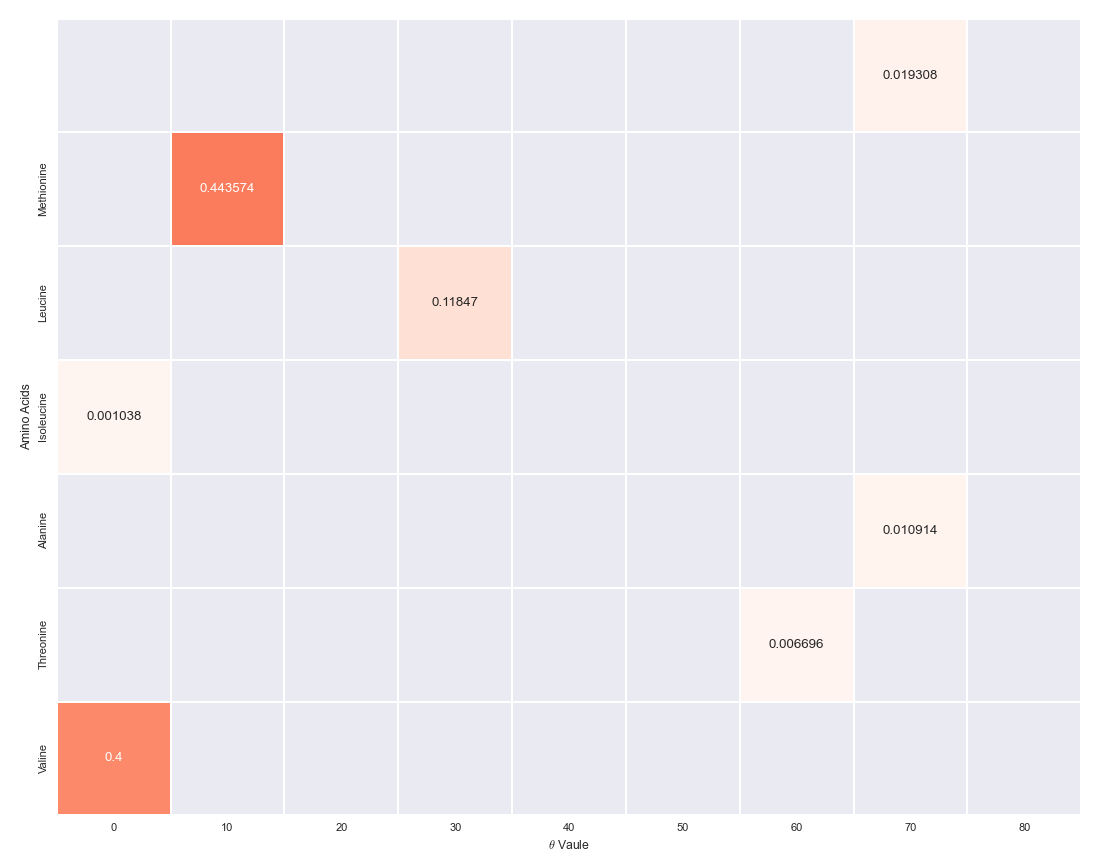
\includegraphics[scale=0.4]{Figures/chapter6_figure_two.png}
\caption{Return composition of Experiment 2 for one random run of experiment set with scaling foctor for mixed amino acids with $\theta$ expended from $0^{\circ}$ to $80^{\circ}$} \label{fig:6.2}
\end{figure}

Moreover, as Equation \ref{eqn:6.3} shows the ratio between the percentage of the selected candidates in the return composition and the target one is the same for all the amino acids. The value of this ratio is $0.6$. When this ratio is added up with the extra variable (referred as slack variable in LP) $0.4$, the total is $1$. As the scaling factors are pre-generated in the experiment set, the value is known, which is $0.6$. In conclusion, the slack variable (SV) is returned by LP. Then the scaling factor (SF) equals to $1 - SV$. From the scaling factor, the ratio between the return composition and the target one is known. At the end, the target composition can be re-built from the ratio and the return composition. The re-constructed target composition matches to the original one. \\

\begin{eqnarray} \label{eqn:6.3}
\frac{0.019308}{0.03218} = \frac{0.443574}{0.73929} = \frac{0.11847}{0.19745} =\frac{0.001038}{0.00173}  = \frac{0.010914}{0.01819} = \frac{0.006696}{0.01116} = 0.6
\end{eqnarray}

\begin{figure}[!ht] 
\centering
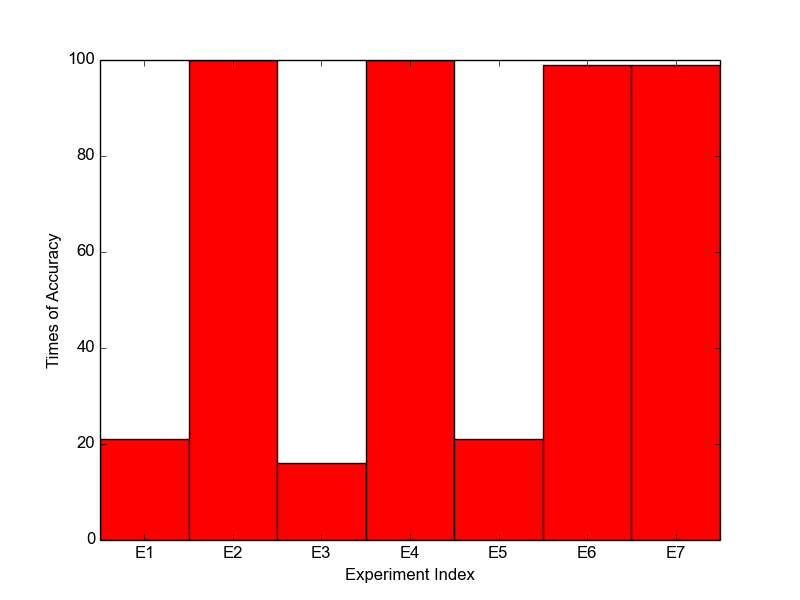
\includegraphics[scale=0.5]{Figures/chapter6_1.png}
\caption{Experiment Accuracy Analysis for Experiments using experimental spectra data that contains scaling factor that is smaller than 1 and candidates with $\theta$ from $0^{\circ}$ to $80^{\circ}$}
\label{fig:6.3}
\end{figure}

To check whether the above observation is a general case, the experiment set in Table \ref{tab:5.1} is run 100 times with randomly generated scaling factors in each run. Figure \ref{fig:6.3} indicates the experiment result. Figure \ref{fig:6.3} shows that Experiment 2, 4, 6 and 7 almost hit the above observation with $100\%$ frequency. This indicates that even with the scaling factor, Raman spectral information alone is sufficient to study the mixed molecules' coordination distribution at interfaces. The target composition can be re-constructed correctly from the return slack variable and the return composition. Figure \ref{fig:6.3} also illustrates that Experiment 3, the LP model with only SFG spectral information, does not hit the above observation with high frequency. With the scaling factor as the addition, SFG spectral information is not sufficient to obtain the target composition. Even combining IR and SFG spectral information, the constructed LP model cannot help to re-construct the target composition. \\

The return slack variable and composition of Experiment 4, 6 and 7 are the same as Experiment 2 in each run. This indicates Raman spectral information are dominating the solution in the LP model. \\

%When the scaling factor is greater than 1, all LP models built by the 7 experiments will fail to obtain the correct composition of target spectrum. (TODO: check with Ulrike and Dennis to see if I need to include this part in my thesis.)\\

When each amino acid's candidates are expanded from $0^{\circ}$ to $180^{\circ}$ on $\theta$, the same experiment set is applied 100 times with randomly generated scaling factors in each run. The result in Figure \ref{fig:6.4} illustrates that none of the experiment in the set meets the observation with high frequency. \\

When the return compositions of Experiment 2 and 6 are further analyzed, there are few observation need to be noticed. To facilitate the explanation, one random run is picked as an explicit example. Figure \ref{fig:6.5} is the target composition. Figure \ref{fig:6.6} is the return composition of Experiment 2. Figure \ref{fig:6.7} is the return composition of Experiment 6. In Figure \ref{fig:6.6}, the slack variable still equals $1 - generated~scaling~factor$. For each amino acid, the selected candidate in the return composition may not be the exact one as the target composition selected. However, this selected candidate is always either the correct one in the target composition, or the correct one's $\theta$ complimentary. In Figure \ref{fig:6.7}, for each amino acid, there are two selected candidates in the return composition. These two selected candidates are the correct one and its $\theta$ complimentary. When the percentages of these two selected candidates are added, it is equalled to the percentage returned for the amino acid in Figure \ref{fig:6.7}. $0.0776716 + 0.0252641 = 0.102936$. Between these two selected candidates, the correct one's percentage is always bigger than its $\theta$ complimentary. $0.0776716 > 0.0252641$. In conclusion, Experiment 2 achieves in telling the slack variable, the scaling factor, and the ratio between the 

The LP model with only Raman spectral information Experiment 2, is able to tell us for each amino acid, candidate with which $\theta$ or this $\theta$'s complementary would exist in our target spectra. Because Raman spectra for candidate with $\theta$ on one degree is the same as its supplementary. This LP model can not distinguish between candidate with $\theta$ and the one with its complementary.However, with the help of SFG, we may be able to know which one between the above two dominates one amino acid's the total fraction, like what we have learnt from Chapter \ref{ch:5} about E6. Therefore we exam E6 here, and it displays which one of the two takes the major composition in the target spectra. With this information, we can decide between the $\theta$ and its complementary. 
With the information coming from E2 and E6, we therefore, obtain the right composition of the target spectrum.\\

Here goes the example, in one run of the experiment group. The composition for the target spectrum is Array \ref{eqn:6.4}. %($result8.txt of result_2016_09_28$)
In this target spectrum, we have 0.14799 of $\theta = 40^{\circ}$ Methionine, 0.74202 of $\theta = 50^{\circ}$ Leucine, 0.08989 of $\theta = 150^{\circ}$ Ile, 0.01135 of $\theta = 40^{\circ}$ Ala, 0.00715 of $\theta = 0^{\circ}$ Thr, 0.0016 of $\theta = 20^{\circ}$ Val. 

\begin{eqnarray}\label{eqn:6.4} 
\resizebox{\linewidth}{!}{$
\begin{bmatrix}
0& 0& 0& 0& 0.14799& 0& 0& 0& 0& 0& 0& 0& 0& 0& 0& 0& 0& 0\\
0& 0& 0& 0& 0& 0.74202& 0& 0& 0& 0& 0& 0& 0& 0& 0& 0& 0& 0\\
0& 0& 0& 0& 0& 0& 0& 0& 0& 0& 0& 0& 0& 0& 0.08989& 0& 0& 0\\
0& 0& 0& 0& 0.01135& 0& 0& 0& 0& 0& 0& 0& 0& 0& 0& 0& 0& 0\\
0.00715& 0& 0& 0& 0& 0& 0& 0& 0& 0& 0& 0& 0& 0& 0& 0& 0& 0\\
0& 0& 0.0016& 0& 0& 0& 0& 0& 0& 0& 0& 0& 0& 0& 0& 0& 0& 0
\end{bmatrix}
$}
\end{eqnarray}

\begin{eqnarray}\label{eqn:6.5} 
\resizebox{\linewidth}{!}{$
\begin{bmatrix}
0& 0& 0& 0& 0.102936& 0& 0& 0& 0& 0& 0& 0& 0& 0& 0& 0& 0& 0\\
0& 0& 0& 0& 0& 0.516118& 0& 0& 0& 0& 0& 0& 0& 0& 0& 0& 0& 0\\
0& 0& 0& 0.0625238& 0& 0& 0& 0& 0& 0& 0& 0& 0& 0& 0& 0& 0& 0\\
0& 0& 0& 0& 0.0078945& 0& 0& 0& 0& 0& 0& 0& 0& 0& 0& 0& 0& 0\\
0.00497324& 0& 0& 0& 0& 0& 0& 0& 0& 0& 0& 0& 0& 0& 0& 0& 0& 0\\
0& 0& 0.00111289& 0& 0& 0& 0& 0& 0& 0& 0& 0& 0& 0& 0& 0& 0& 0\\
0.304441
\end{bmatrix}
$}
\end{eqnarray}
The result returned by E2 is shown in Array \ref{eqn:6.5}. You may notice same as Array \ref{eqn:6.2} to Array \ref{eqn:6.1}, Array \ref{eqn:6.5} contains one more value than Array \ref{eqn:6.4}, 0.304441, which is the slack variable. We already know that the scaling factor is 0.695560510845(generated randomly, but recorded). When we add the slack variable and the scaling factor, the total comes up to 1.0. \\

In Array \ref{eqn:6.5}, we get 0.102936 of $\theta = 40^{\circ}$ Methionine, 0.516118 of $\theta = 50^{\circ}$ Leucine, 0.0625238 of $\theta = 30^{\circ}$ Ile, 0.0078945 of $\theta = 40^{\circ}$ Ala, 0.00497324 of $\theta = 0^{\circ}$ Thr, 0.00111289 of $\theta = 20^{\circ}$ Val. From Array \ref{eqn:6.6}, we can also deduce the value for the scaling factor.

\begin{eqnarray} \label{eqn:6.6}
\begin{split}
\frac{0.102936}{0.14799} &= \frac{0.516118}{0.74202} = \frac{0.0625238}{0.08989}  =\frac{0.0078945}{0.01135}  
\\
\\
&= \frac{0.00497324}{0.00715} = \frac{0.00111289}{0.0016} = 0.695560
\end{split}
\end{eqnarray}


At first glance, we may guess that this LP model actually return the correct composition. However, not all amino acids' composition is correct. For Ile, it should be 0.0625238 of $\theta = 150^{\circ}$, but the result returned 0.0625238 of $\theta = 30^{\circ}$, which is the complimentary of $150^{\circ}$. It is because these two degrees' Raman spectra are identical, there is no way for current LP model to distinguish these two. \\

With this information, we know the only thing we need to make sure is: is the $\theta$ returned by LP model the exact one in target spectrum or its complementary? (The above conclusion can also be applied to the experiments in Chapter \ref{ch:5} without the scaling factor. The LP model with only Raman spectra information can help us to see which $\theta$ of candidate and its complimentary should be for each amino acid. I did not observe this before.)\\

To answer this question, we need the help of SFG data. Because only SFG can tell us the difference between one angle and its complementary, as their spectra are symmetry, not identical around the axis of wevenumber.\\

In this experiment group, the result returned E6 is Array \ref{eqn:6.7}  (Second example???)
\begin{eqnarray}\label{eqn:6.7} 
\resizebox{\linewidth}{!}{$
\begin{bmatrix}
0& 0& 0& 0& 0.0776716& 0& 0& 0& 0& 0& 0& 0& 0& 0.0252641& 0& 0& 0& 0     \\
0& 0& 0& 0& 0& 0.3894440& 0& 0& 0& 0& 0& 0& 0.1266740& 0& 0& 0& 0& 0     \\
0& 0& 0& 0.0153456& 0& 0& 0& 0& 0& 0& 0& 0& 0& 0& 0.0471782& 0& 0& 0     \\
0& 0& 0& 0& 0.00595697& 0& 0& 0& 0& 0& 0& 0& 0& 0.00193762& 0& 0& 0& 0   \\
0.0037526& 0& 0& 0& 0& 0& 0& 0& 0& 0& 0& 0& 0& 0& 0& 0& 0& 0.00122061    \\
0& 0& 0.000839749& 0& 0& 0& 0& 0& 0& 0& 0& 0& 0& 0& 0& 0.000273144& 0& 0 \\
0.304441 (any relation for the fraction???)
\end{bmatrix}
$}
\end{eqnarray}

The value of the slack variable is the same as what returned by E2. However, the returned composition is totally different than what returned by E2. The interesting thing is that for each amino acid, the return existing candidates are complementary on $\theta$. The total percentage of these two candidates, take Methionine as an instance, $0.0776716 + 0.0252641$ makes 0.1029357 which is the same as what is returned by E2. This is the same for every amino acid. What's more, the composition returned by the E6 indicates which $\theta$ dominates the composition for one amino acid. For Methionine, $\theta = 40^{\circ}$ takes major part; for Leucine, $\theta = 50^{\circ}$ does; for Ile, $\theta = 30^{\circ}$ does; for Ala, $\theta = 40^{\circ}$ does; for Thr, $\theta = 0^{\circ}$  does; for Val, $\theta = 20^{\circ}$ does; And those candidates are the correct components for target spectra. 




IR+SFG, can you do anything with it???




\section{Results}
\section{Discussion}
\section{Conclusions}
\label{experimental}


